\documentclass[tikz,convert={density=150,size=600,outext=.png}]{standalone}
\usetikzlibrary{shapes, calc, arrows, fit, positioning, decorations, patterns, decorations.pathreplacing, chains, snakes}

\begin{document}
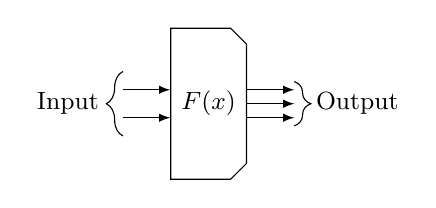
\begin{tikzpicture}[>=latex, scale=0.6, font=\small]
\node[draw, chamfered rectangle, chamfered rectangle corners={north east, south east}, inner ysep=0.7cm, inner xsep=1pt] (fx) {$F(x)$};

\draw[->] ([xshift=-1cm] fx.160) -- (fx.160);
\draw[->] ([xshift=-1cm] fx.200) -- (fx.200);
\draw[decorate, decoration={brace, amplitude=6pt}] ([xshift=-1.cm] fx.220) -- ([xshift=-1.cm] fx.140) node[midway, xshift=-0.7cm] {Input};

\draw[->] (fx.20) -- ([xshift=1cm] fx.20);
\draw[->] (fx.0) -- ([xshift=1cm] fx.0);
\draw[->] (fx.340) -- ([xshift=1cm] fx.340);

\draw[decorate, decoration={brace, amplitude=6pt}] ([xshift=1.cm] fx.30) -- ([xshift=1.cm] fx.330) node[midway, xshift=0.8cm] {Output};
\end{tikzpicture}
\end{document}
